
\documentclass[tikz, border=10pt]{standalone}

\usepackage{verbatim}
\usepackage{amsmath}

\tikzset{>=stealth}
\tikzstyle{every node}=[align=center]

\begin{document}
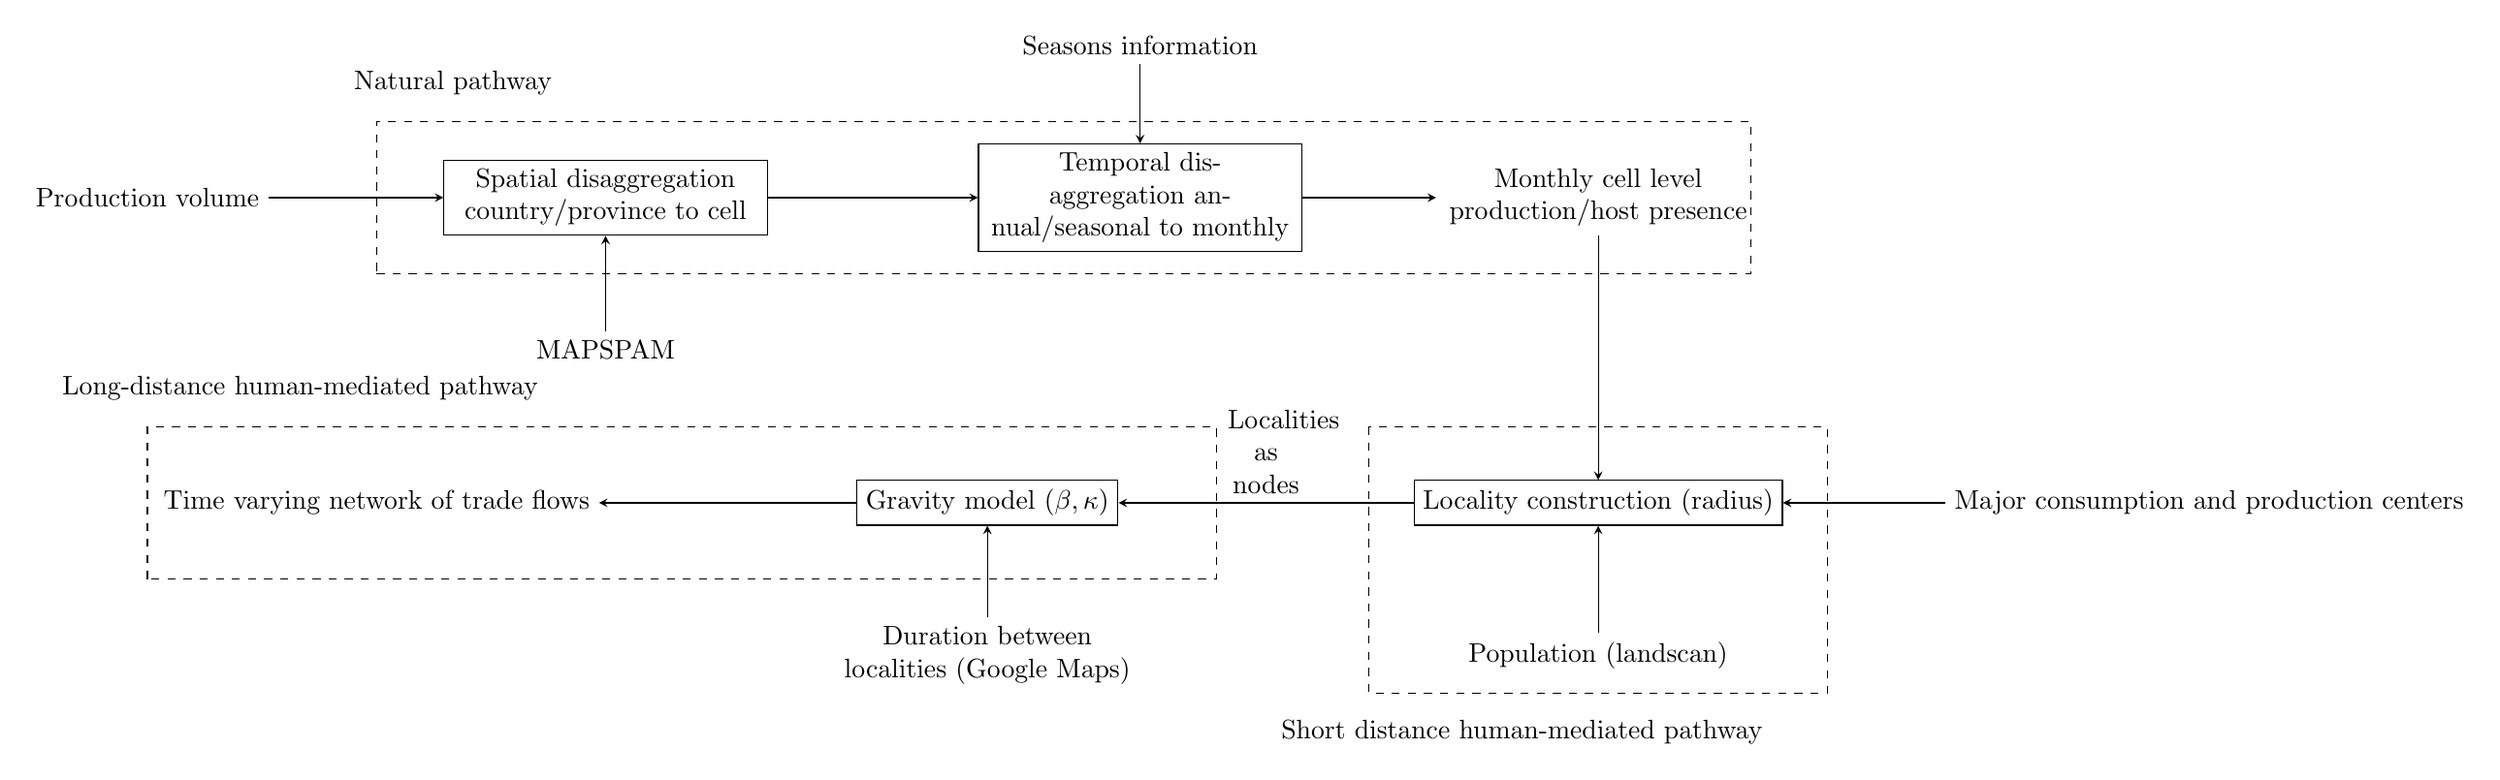
\begin{tikzpicture}

\node[draw] (spatial) [text width=4cm] at (-2,2) {Spatial disaggregation country/province to cell};
\node (prod) at (-8,2) {Production volume};
\node (mapspam) at (-2,0) {MAPSPAM};
\node (natural) at (-4,3.5) {Natural pathway};
\node[draw, text width=4cm] (temporal) at (5, 2) {Temporal disaggregation annual/seasonal to monthly};
\node (seasons) at (5, 4) {Seasons information};
\node (monthly) [text width=4cm] at (11,2) {Monthly cell level production/host presence};
\node[draw] (locality) at (11, -2) {Locality construction (radius)};
\node (major) at (19, -2) {Major consumption and production centers};
\node (population) at (11, -4) {Population (landscan)};
\node[draw] (gravity) at (3, -2) {Gravity model ($\beta ,\kappa$)};
\node[text width=4cm] (duration) at (3, -4) {Duration between localities (Google Maps)};
\node (network) at (-5, -2) {Time varying network of trade flows};
\node (pathway) at (-6, -0.5) {Long-distance human-mediated pathway};
\node (short path) at (10, -5) {Short distance human-mediated pathway};

\draw[dashed] (-5,1) -- (13,1) -- (13,3) -- (-5,3) -- (-5,1);
\draw[dashed] (-8,-3) -- (-8,-1) -- (6,-1) -- (6,-3) -- (-8,-3);
\draw[dashed] (8,-1) -- (8,-4.5) --(14,-4.5) -- (14,-1) -- (8,-1);
\draw[->] (prod) to (spatial);
\draw[->] (mapspam) to (spatial);
\draw[->] (spatial) to (temporal);
\draw[->] (seasons) to (temporal);
\draw[->] (temporal) to (monthly);
\draw[->] (monthly) to (locality);
\draw[->] (major) to (locality);
\draw[->] (population) to (locality);
\draw[->] (locality) to node[above,text width=1cm] {Localities as nodes} (gravity);
\draw[->] (duration) to (gravity);
\draw[->] (gravity) to (network);
% \draw[->] (network) to (pathway);
 



  % Dialectics
%  \node[draw] (Thesis) at (0,0) {Thesis};
%  \node[draw,fill=black,text=white] (Antithesis) at (2.3,0) {Antithesis};
%  \node[draw,fill=gray,text=white] (Synthesis) at (1,2) {Synthesis};
%  
%  
%
%  \draw[->,draw=blue] (Synthesis) to[in=180,out=180] (Thesis);
%  
%  \node at (1.0, -1.0) {\textit{a) Dialectics}};
%  
%  % Opposition
%  \node[draw] (ArgumentA) at (5,0) {Argument};
%  \node[draw,fill=black,text=white] (ArgumentB) at (7.5,0) {Opposition};
%  
%  \draw[->,draw=blue] (ArgumentA) to (ArgumentB);
%  
%  \node at (6., -1.0) {\textit{b) Opposition}};
%  
%  % Innovation
%  \node[draw] (ArgumentA) at (10.1,0) {Argument};
%  \node[draw,fill=black,text=white] (ArgumentB) at (13,0) {Opposition};
%  \node[draw,fill=yellow] (ArgumentC) at (12,2) {Innovation};
%  
%
%  
%  \node at (11.5, -1.0) {\textit{c) Innovation}};
\end{tikzpicture}
\end{document}